Para este punto se desarrollaron nuevas instancias random distintas a las anteriores. La generación de nuevos casos de prueba es debido a que los anteriormente utilizados podrían formar una muestra aleatoria que beneficiase más a ciertos algoritmos que a otros. De esta forma podremos evidenciar las diferencias que haya entre las distintas aproximaciones.

El siguiente es un ejemplo de una instancia dentro de este conjunto nuevo, ejecutada en las 5 variantes:

\vspace*{0.3cm} \vspace*{0.3cm}
  \begin{center}
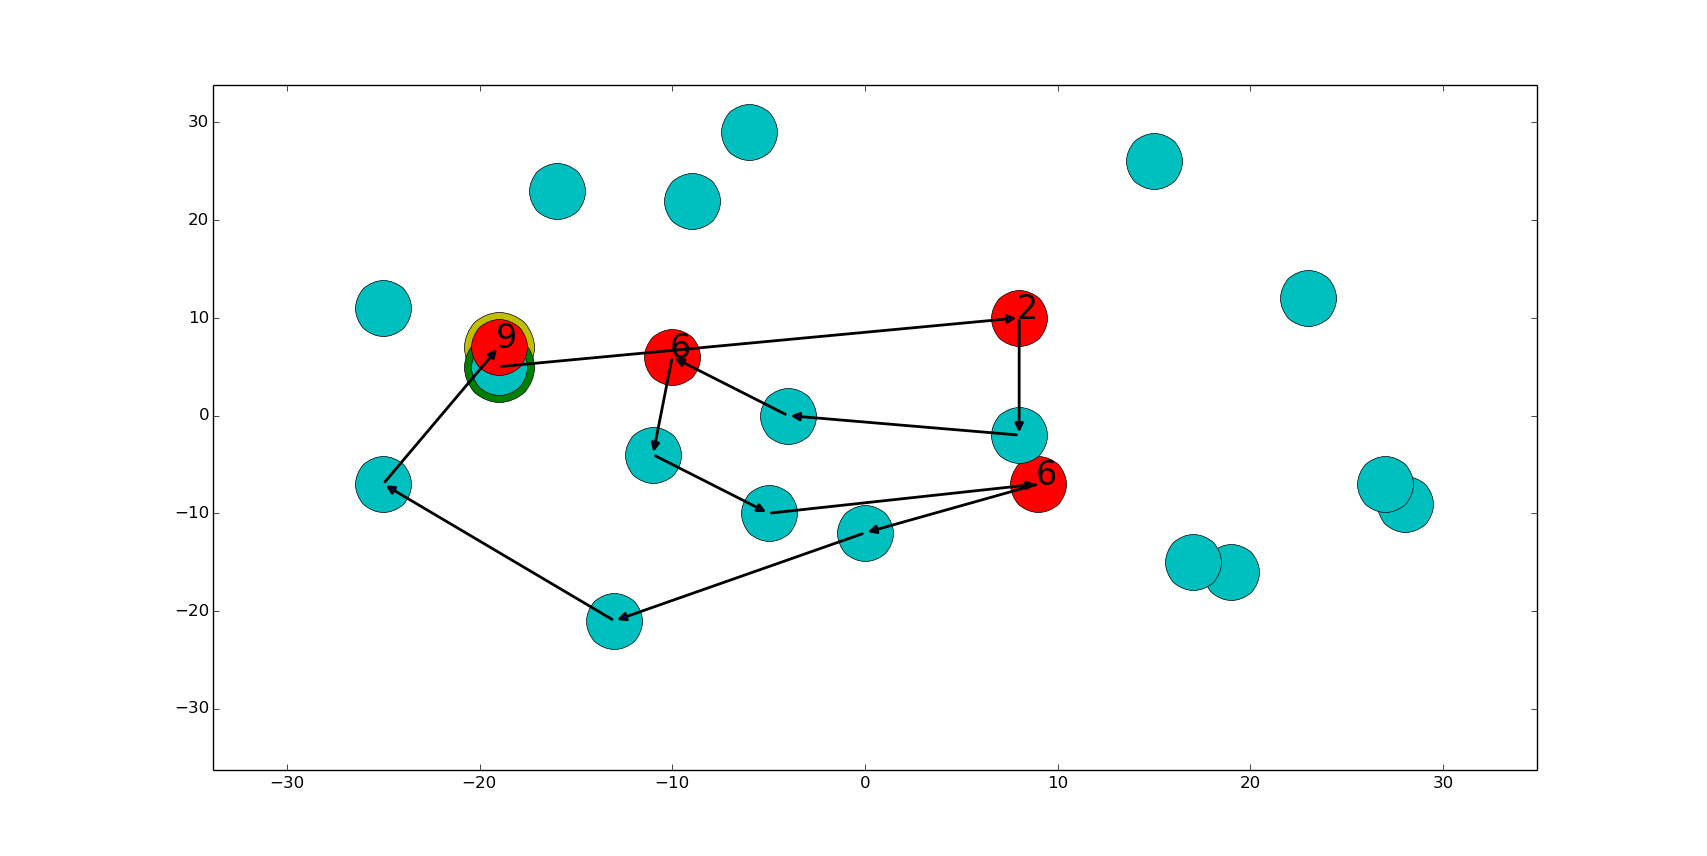
\includegraphics[scale=0.3]{./EJ5/caminoEjGoloso.png}
\\{\textit{Resultado goloso}}
  \end{center}
  \vspace*{0.3cm}
  
  \vspace*{0.3cm} \vspace*{0.3cm}
  \begin{center}
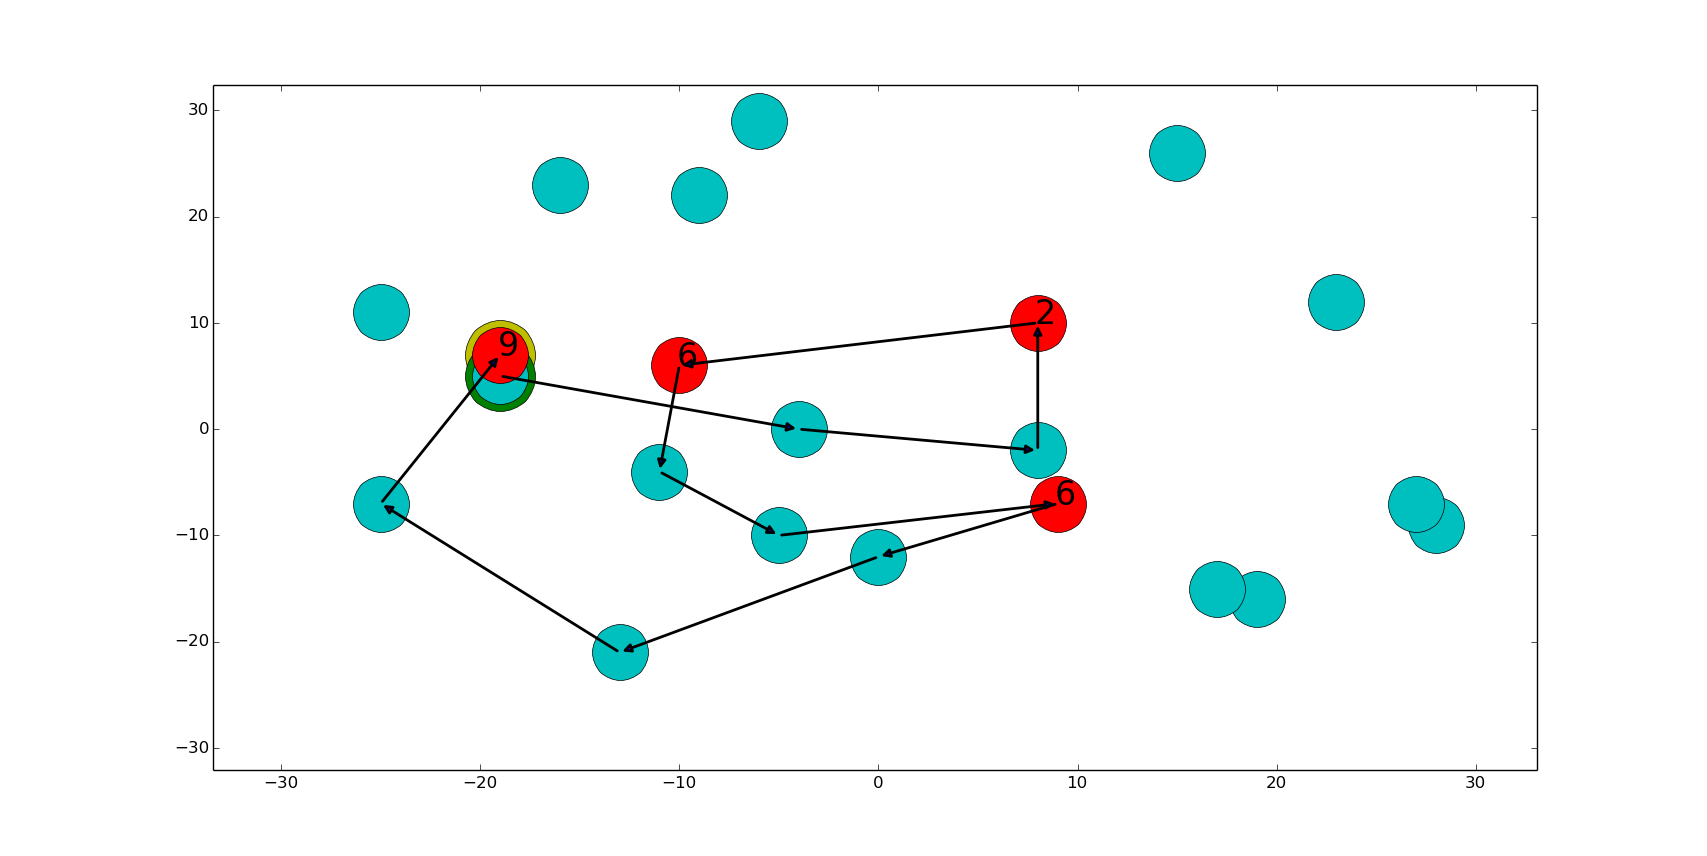
\includegraphics[scale=0.3]{./EJ5/caminoEjswap.png}
\\{\textit{Resultado SWAP}}
  \end{center}
  \vspace*{0.3cm}

  \vspace*{0.3cm} \vspace*{0.3cm}
  \begin{center}
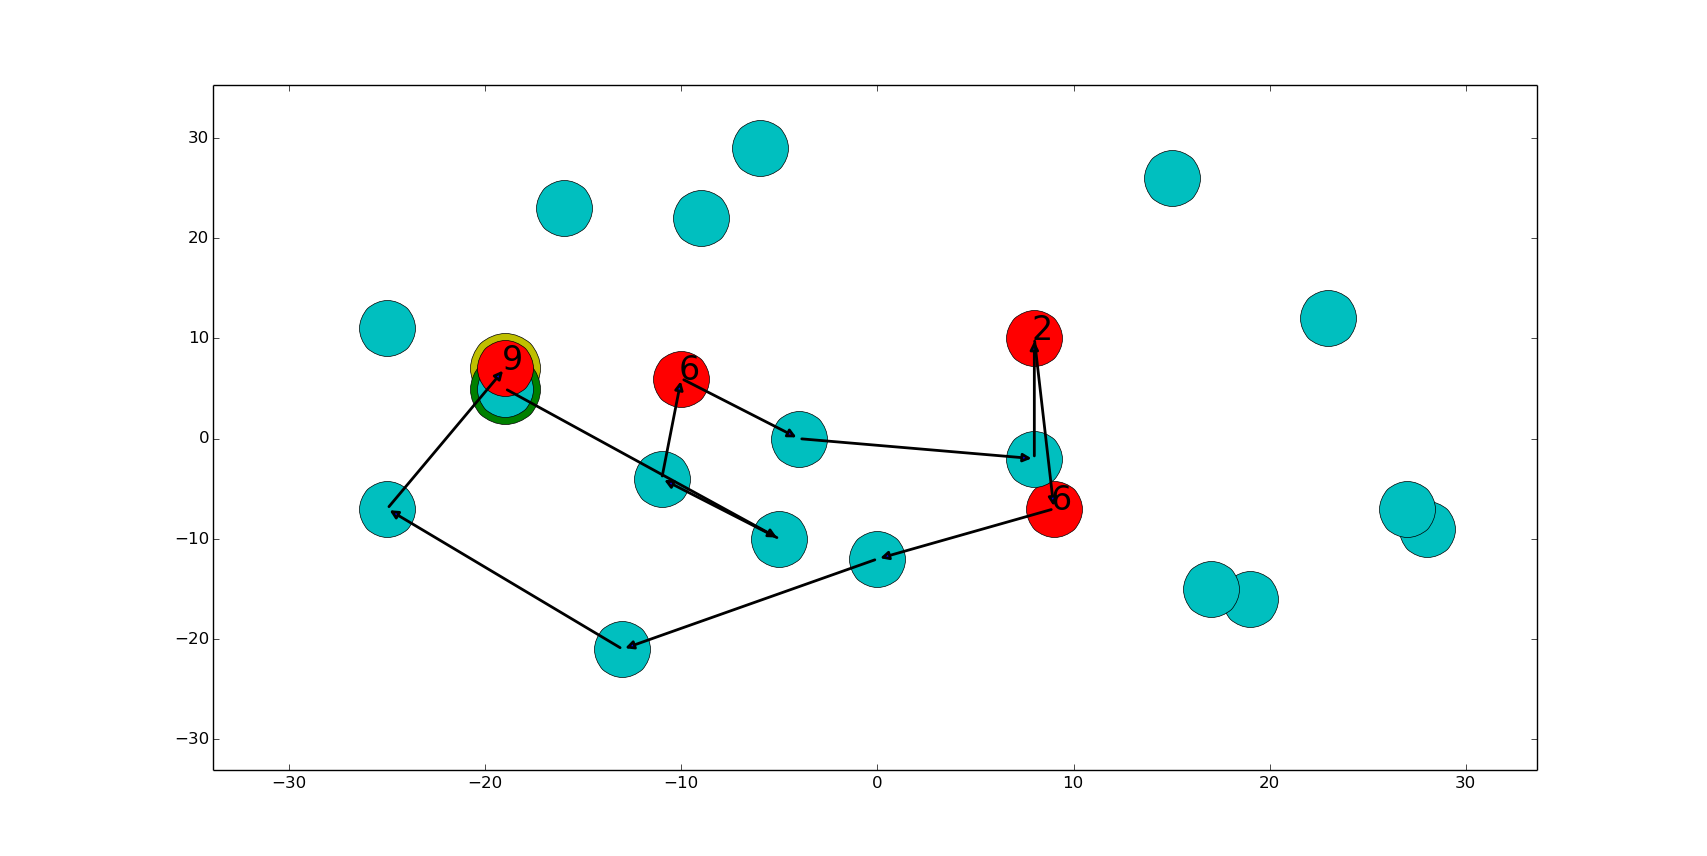
\includegraphics[scale=0.3]{./EJ5/caminoEj2opt.png}
\\{\textit{Resultado 2-OPT}}
  \end{center}
  \vspace*{0.3cm}
  
    \vspace*{0.3cm} \vspace*{0.3cm}
  \begin{center}
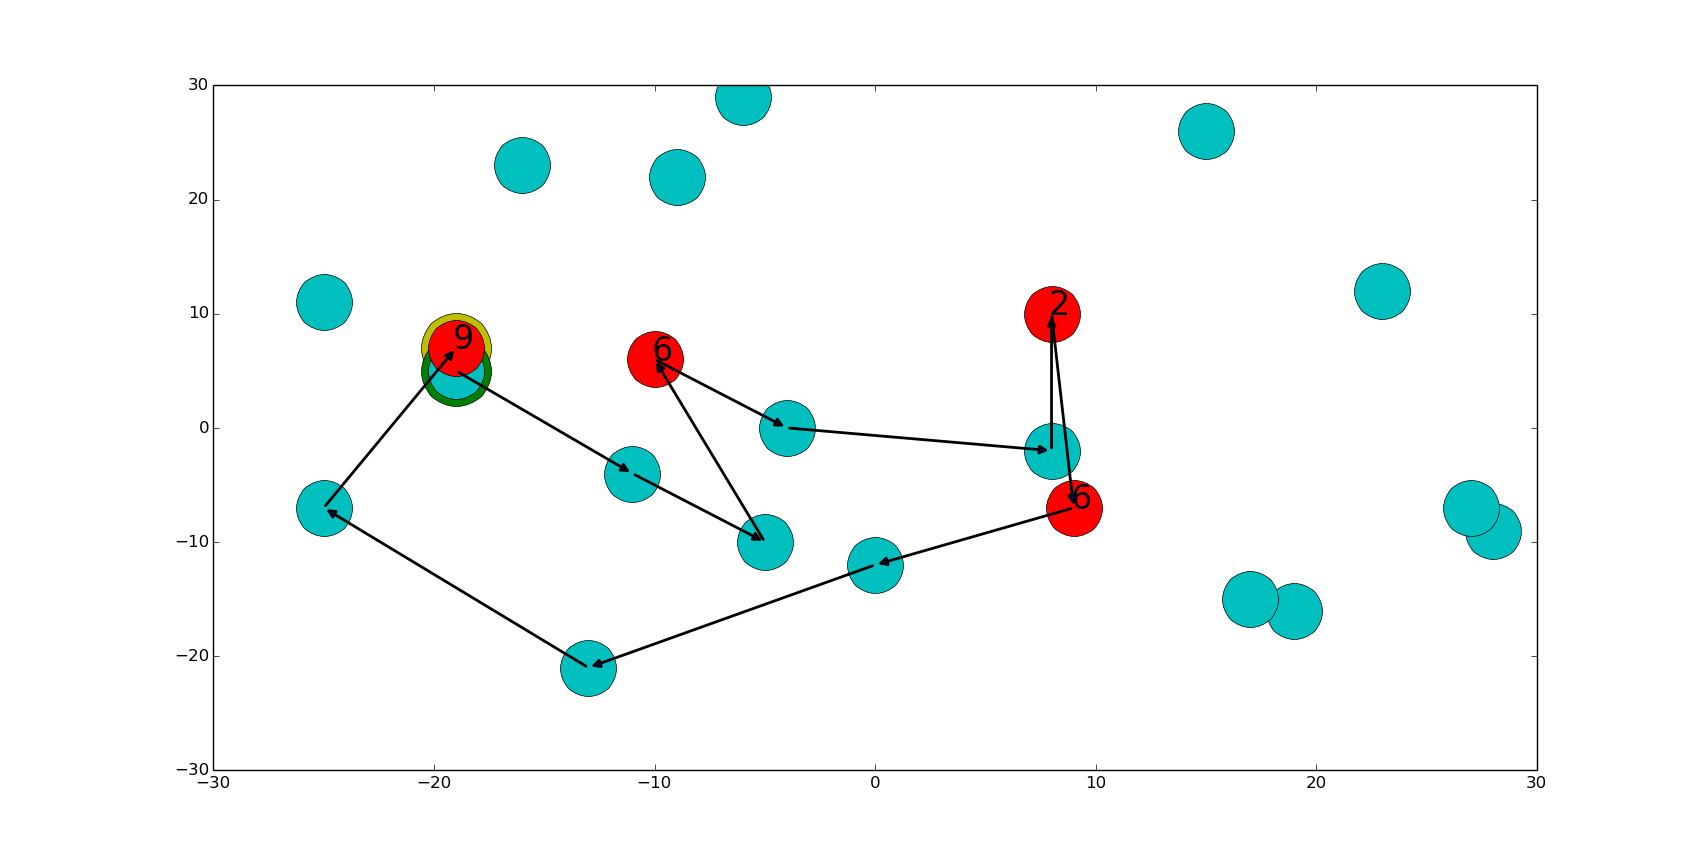
\includegraphics[scale=0.3]{./EJ5/caminoEj3opt.png}
\\{\textit{Resultado 3-OPT}}
  \end{center}
  \vspace*{0.3cm}

\subsubsection{Comparaciones de tiempo entre heuristicas}

Para corroborar la performance obtenida para este grupo de instancias se tomaron los tiempos que tarda cada algoritmo de busqueda local en obtener soluci\'on. 
Dicho conjunto esta formado por un total de 50 instancias que van desde 2 elementos hasta 50 en total.

-----> GRAFICO DE MEDICIONES 
\vspace*{0.3cm} \vspace*{0.3cm}
  \begin{center}
 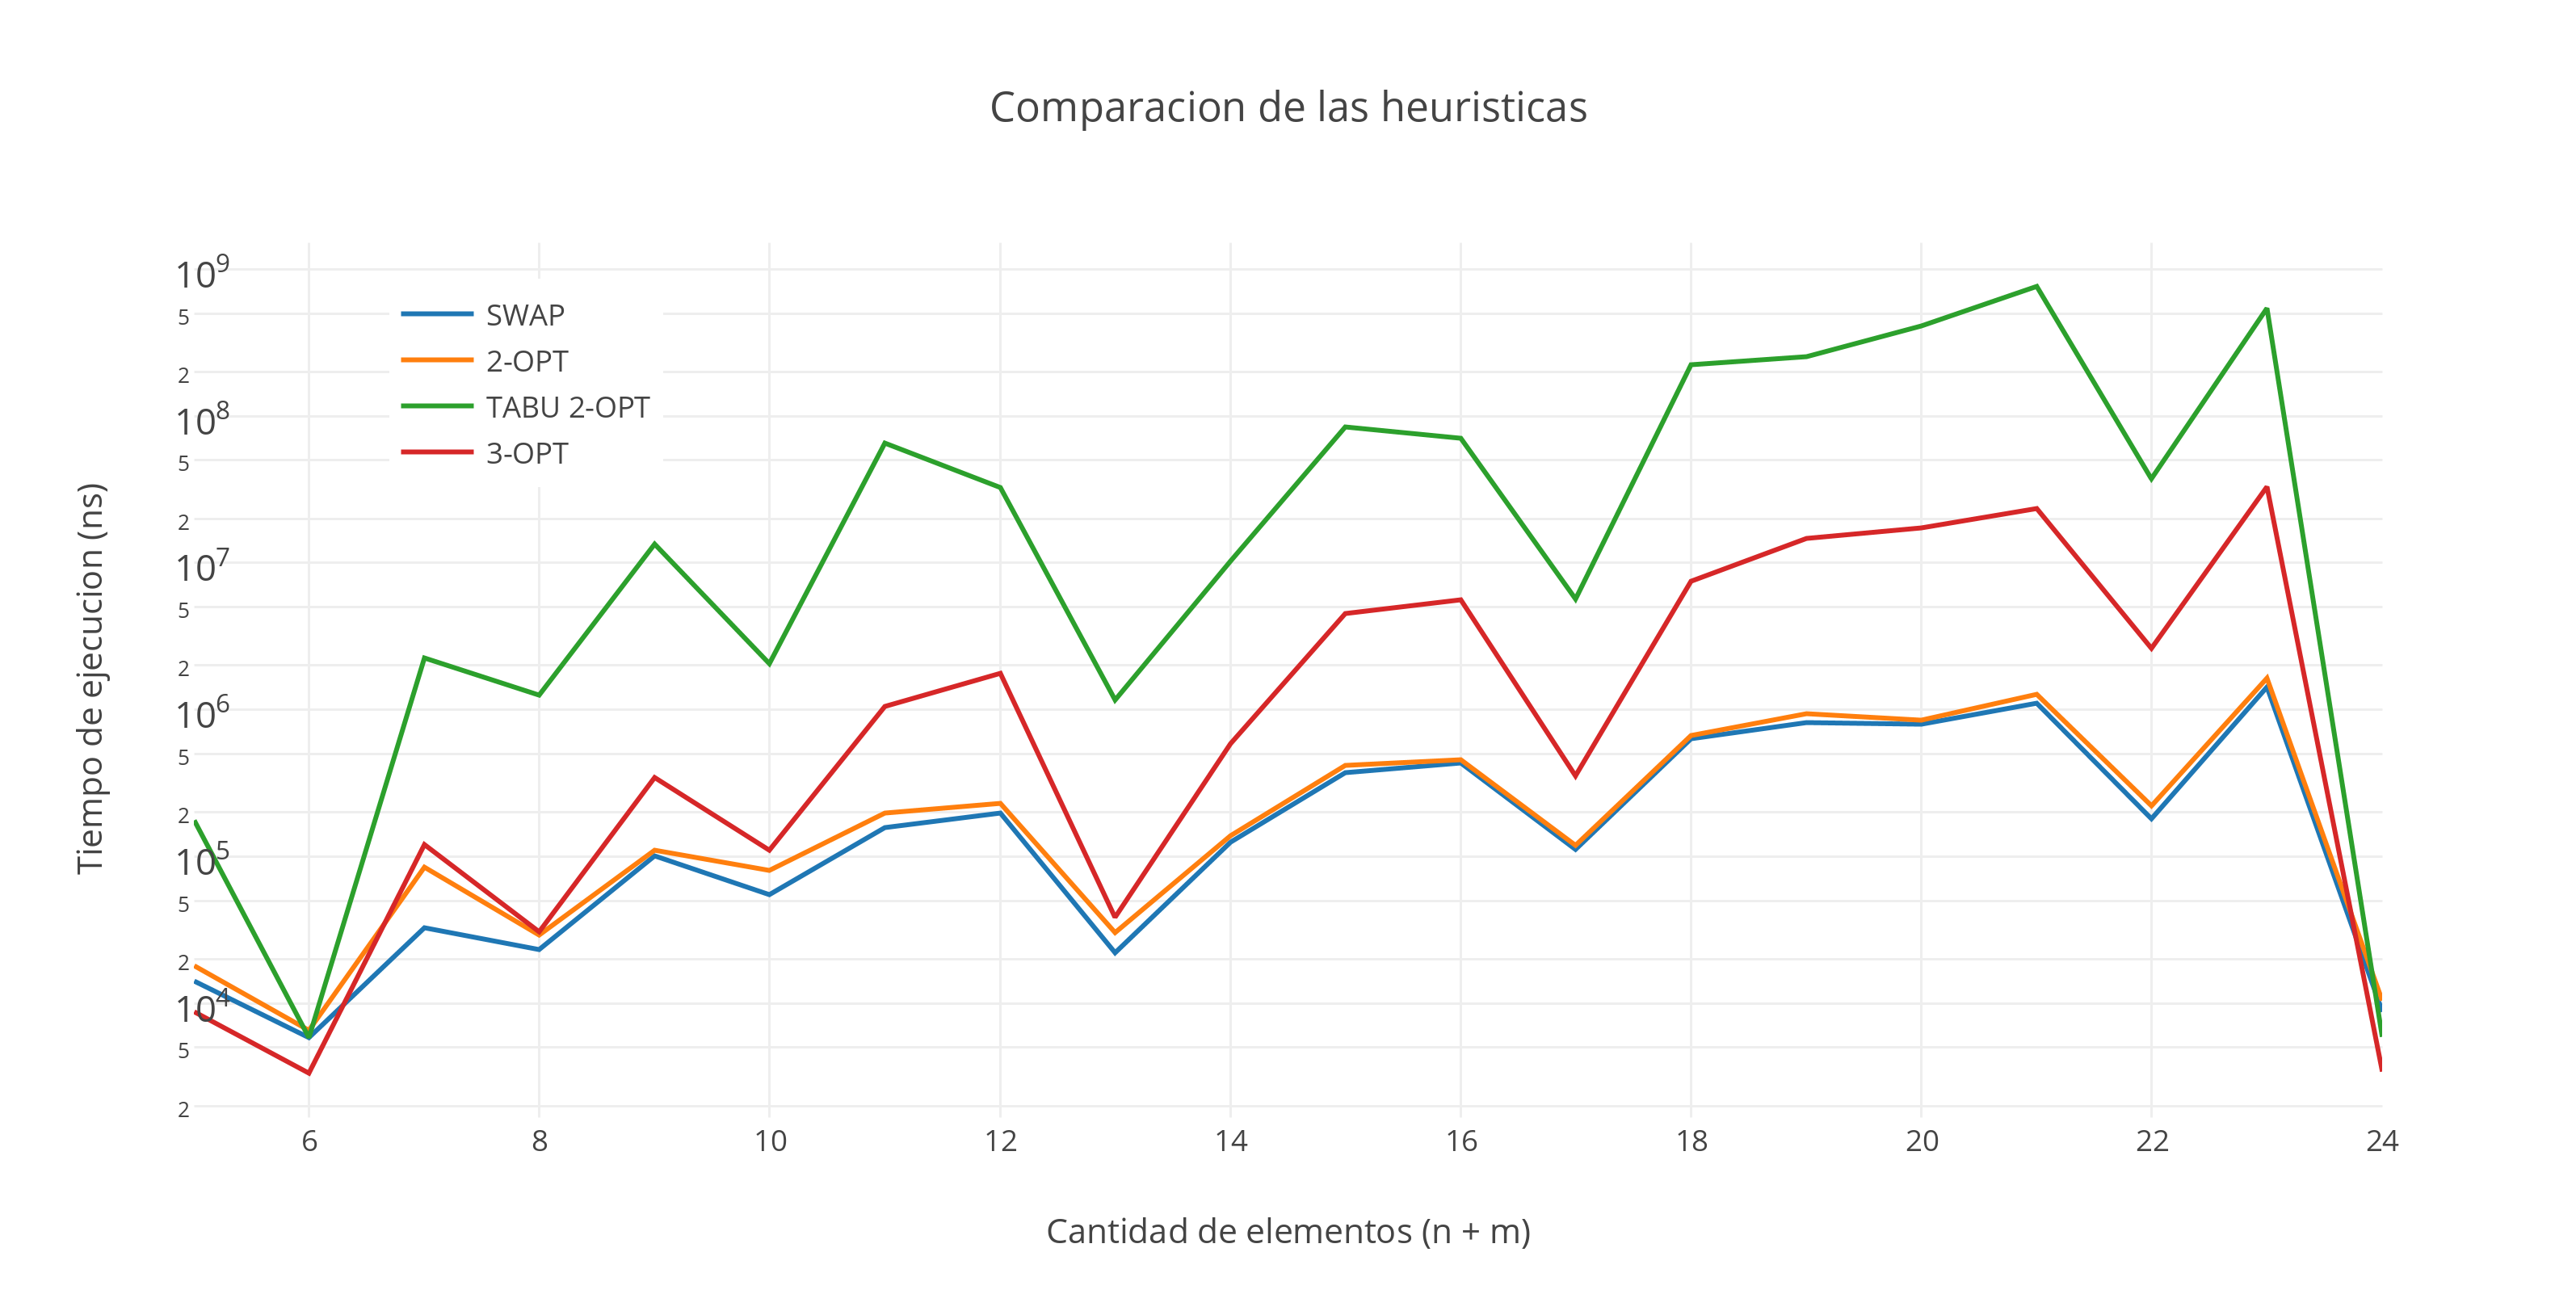
\includegraphics[scale=0.5]{./EJ5/medicion.png}\\
 {\textit{Gráfico \ 5.1 - Performance de las Heur\'isticas}}
  \end{center}
  \vspace*{0.3cm}


Podemos ver que las busquedas locales que se efectuan en menor tiempo son SWAP y 2-OPT. 
Al igual que en los anteriores conjuntos de instancias.

-----> GRAFICO DE MEDICIONES 
\vspace*{0.3cm} \vspace*{0.3cm}
  \begin{center}
 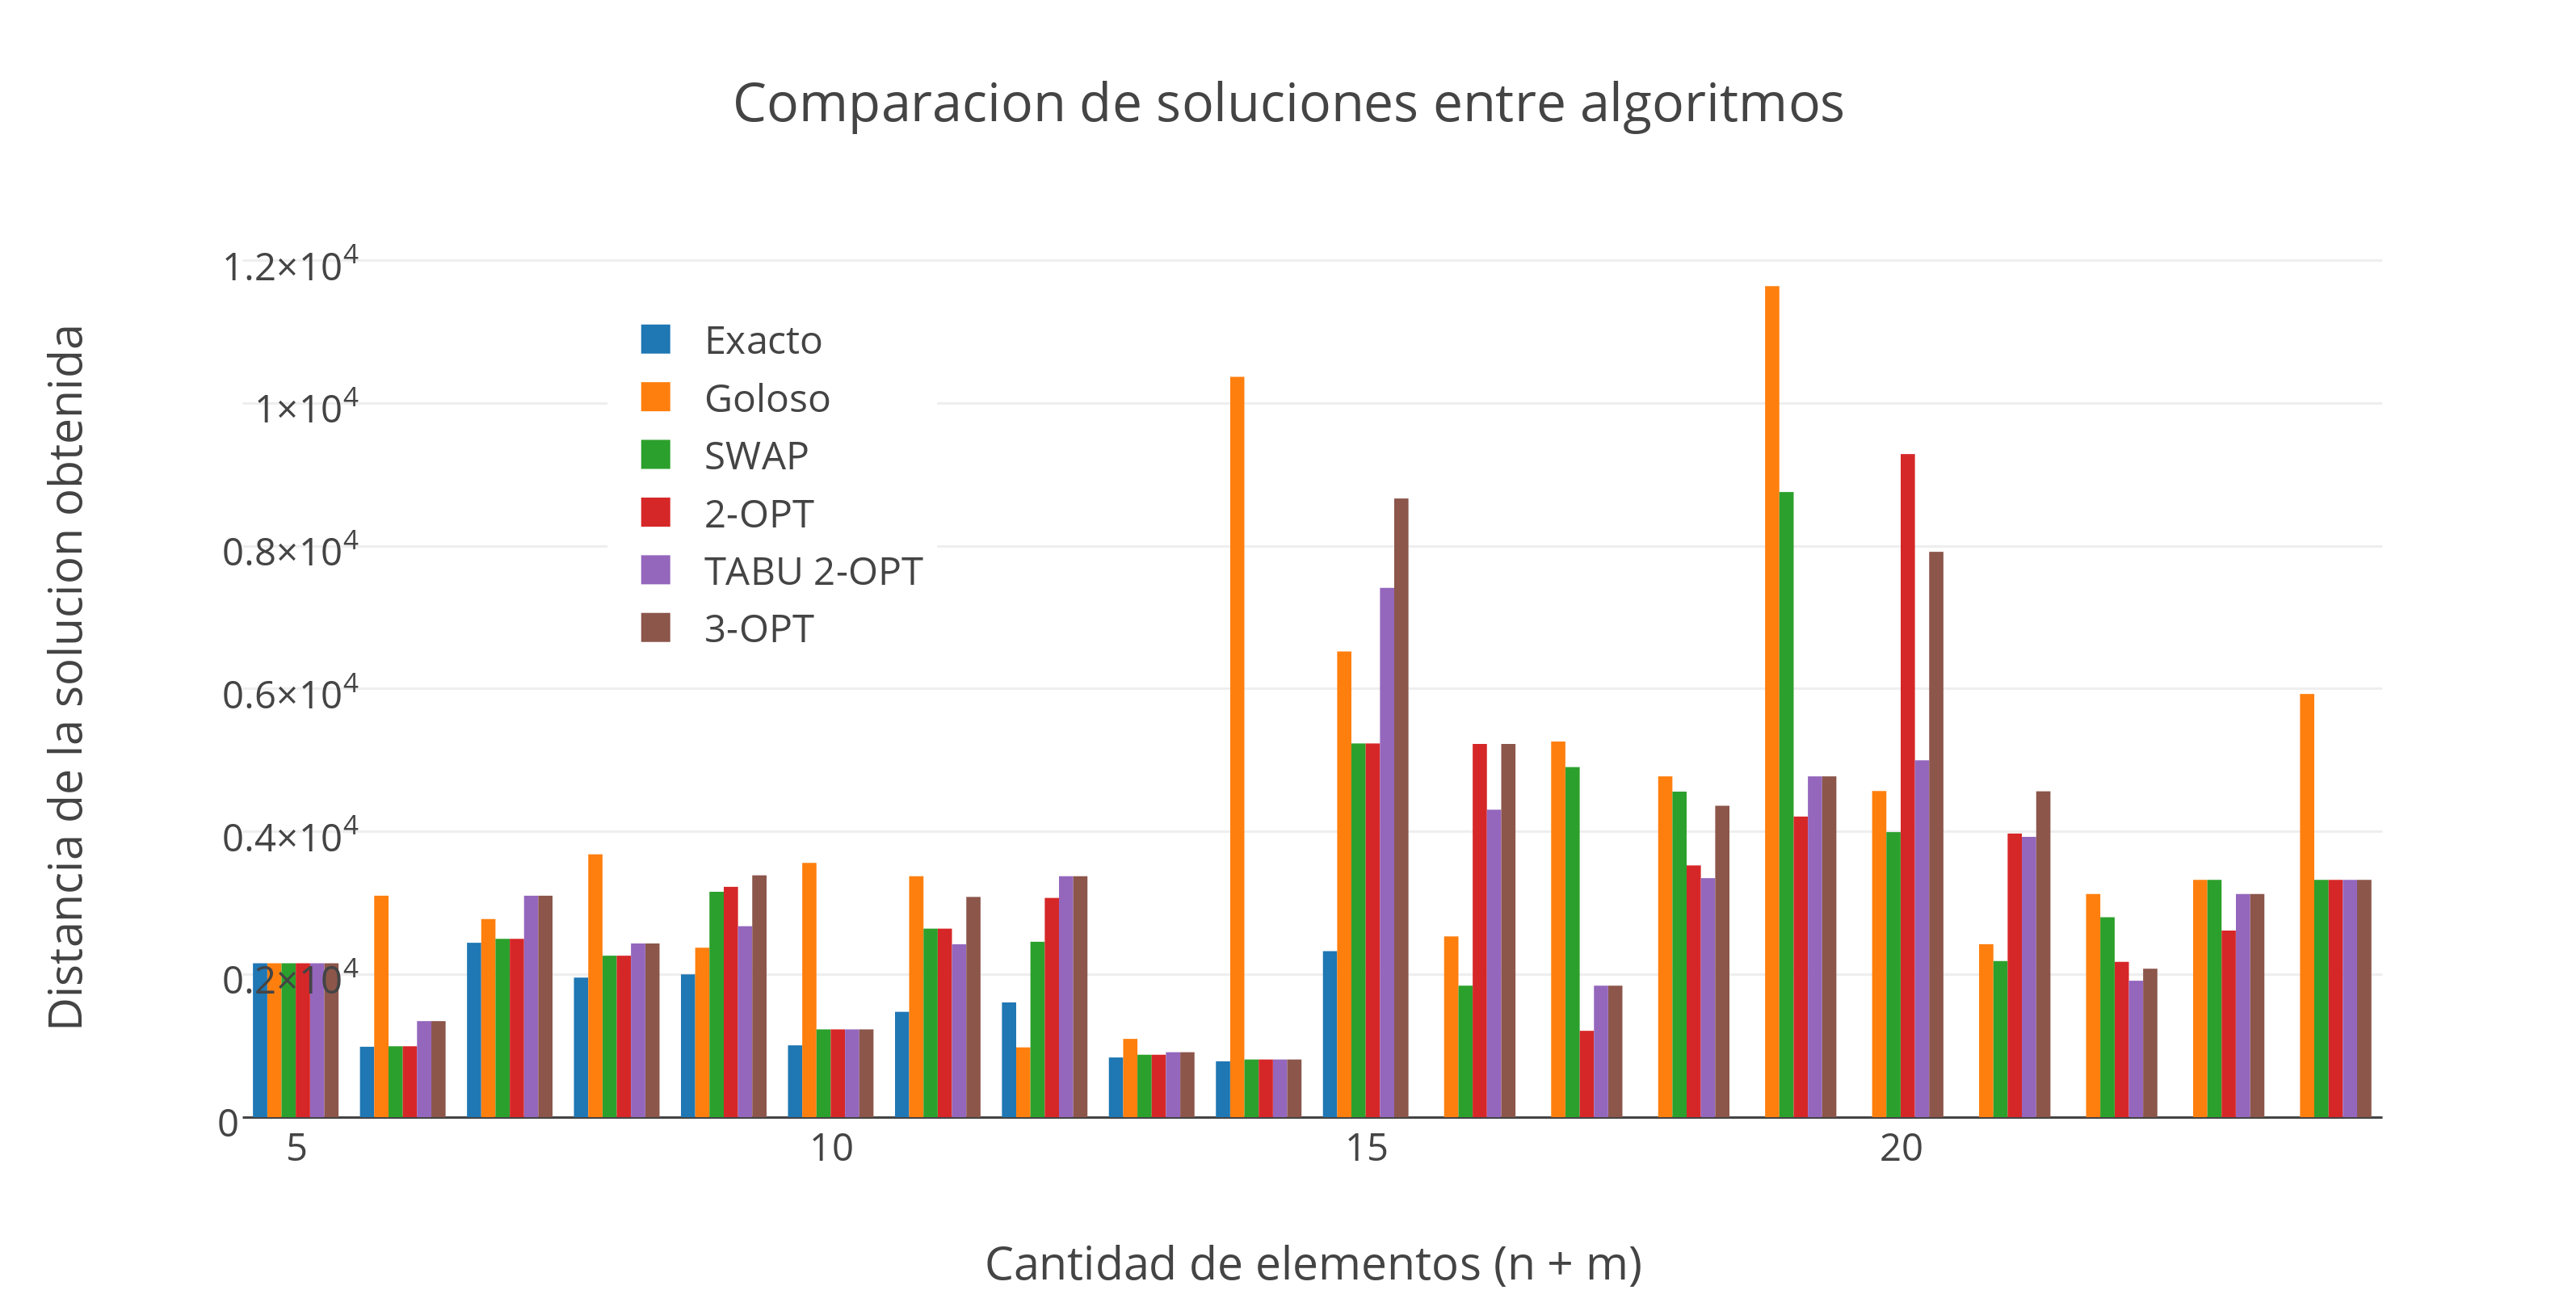
\includegraphics[scale=0.5]{./EJ5/comparativo.png}\\
 {\textit{Gráfico \ 5.2 - Comparaci\'on de soluciones de todos los algoritmos}}
  \end{center}
  \vspace*{0.3cm}

Se realizo una primera comparaci\'on entre las heur\'isticas y el backtraking tomando las primeras 20 instancias que son v\'alidas para ser ejecutadas para una mejor visualizaci\'on de los resultados.

\vspace*{0.3cm} \vspace*{0.3cm}
  \begin{center}
 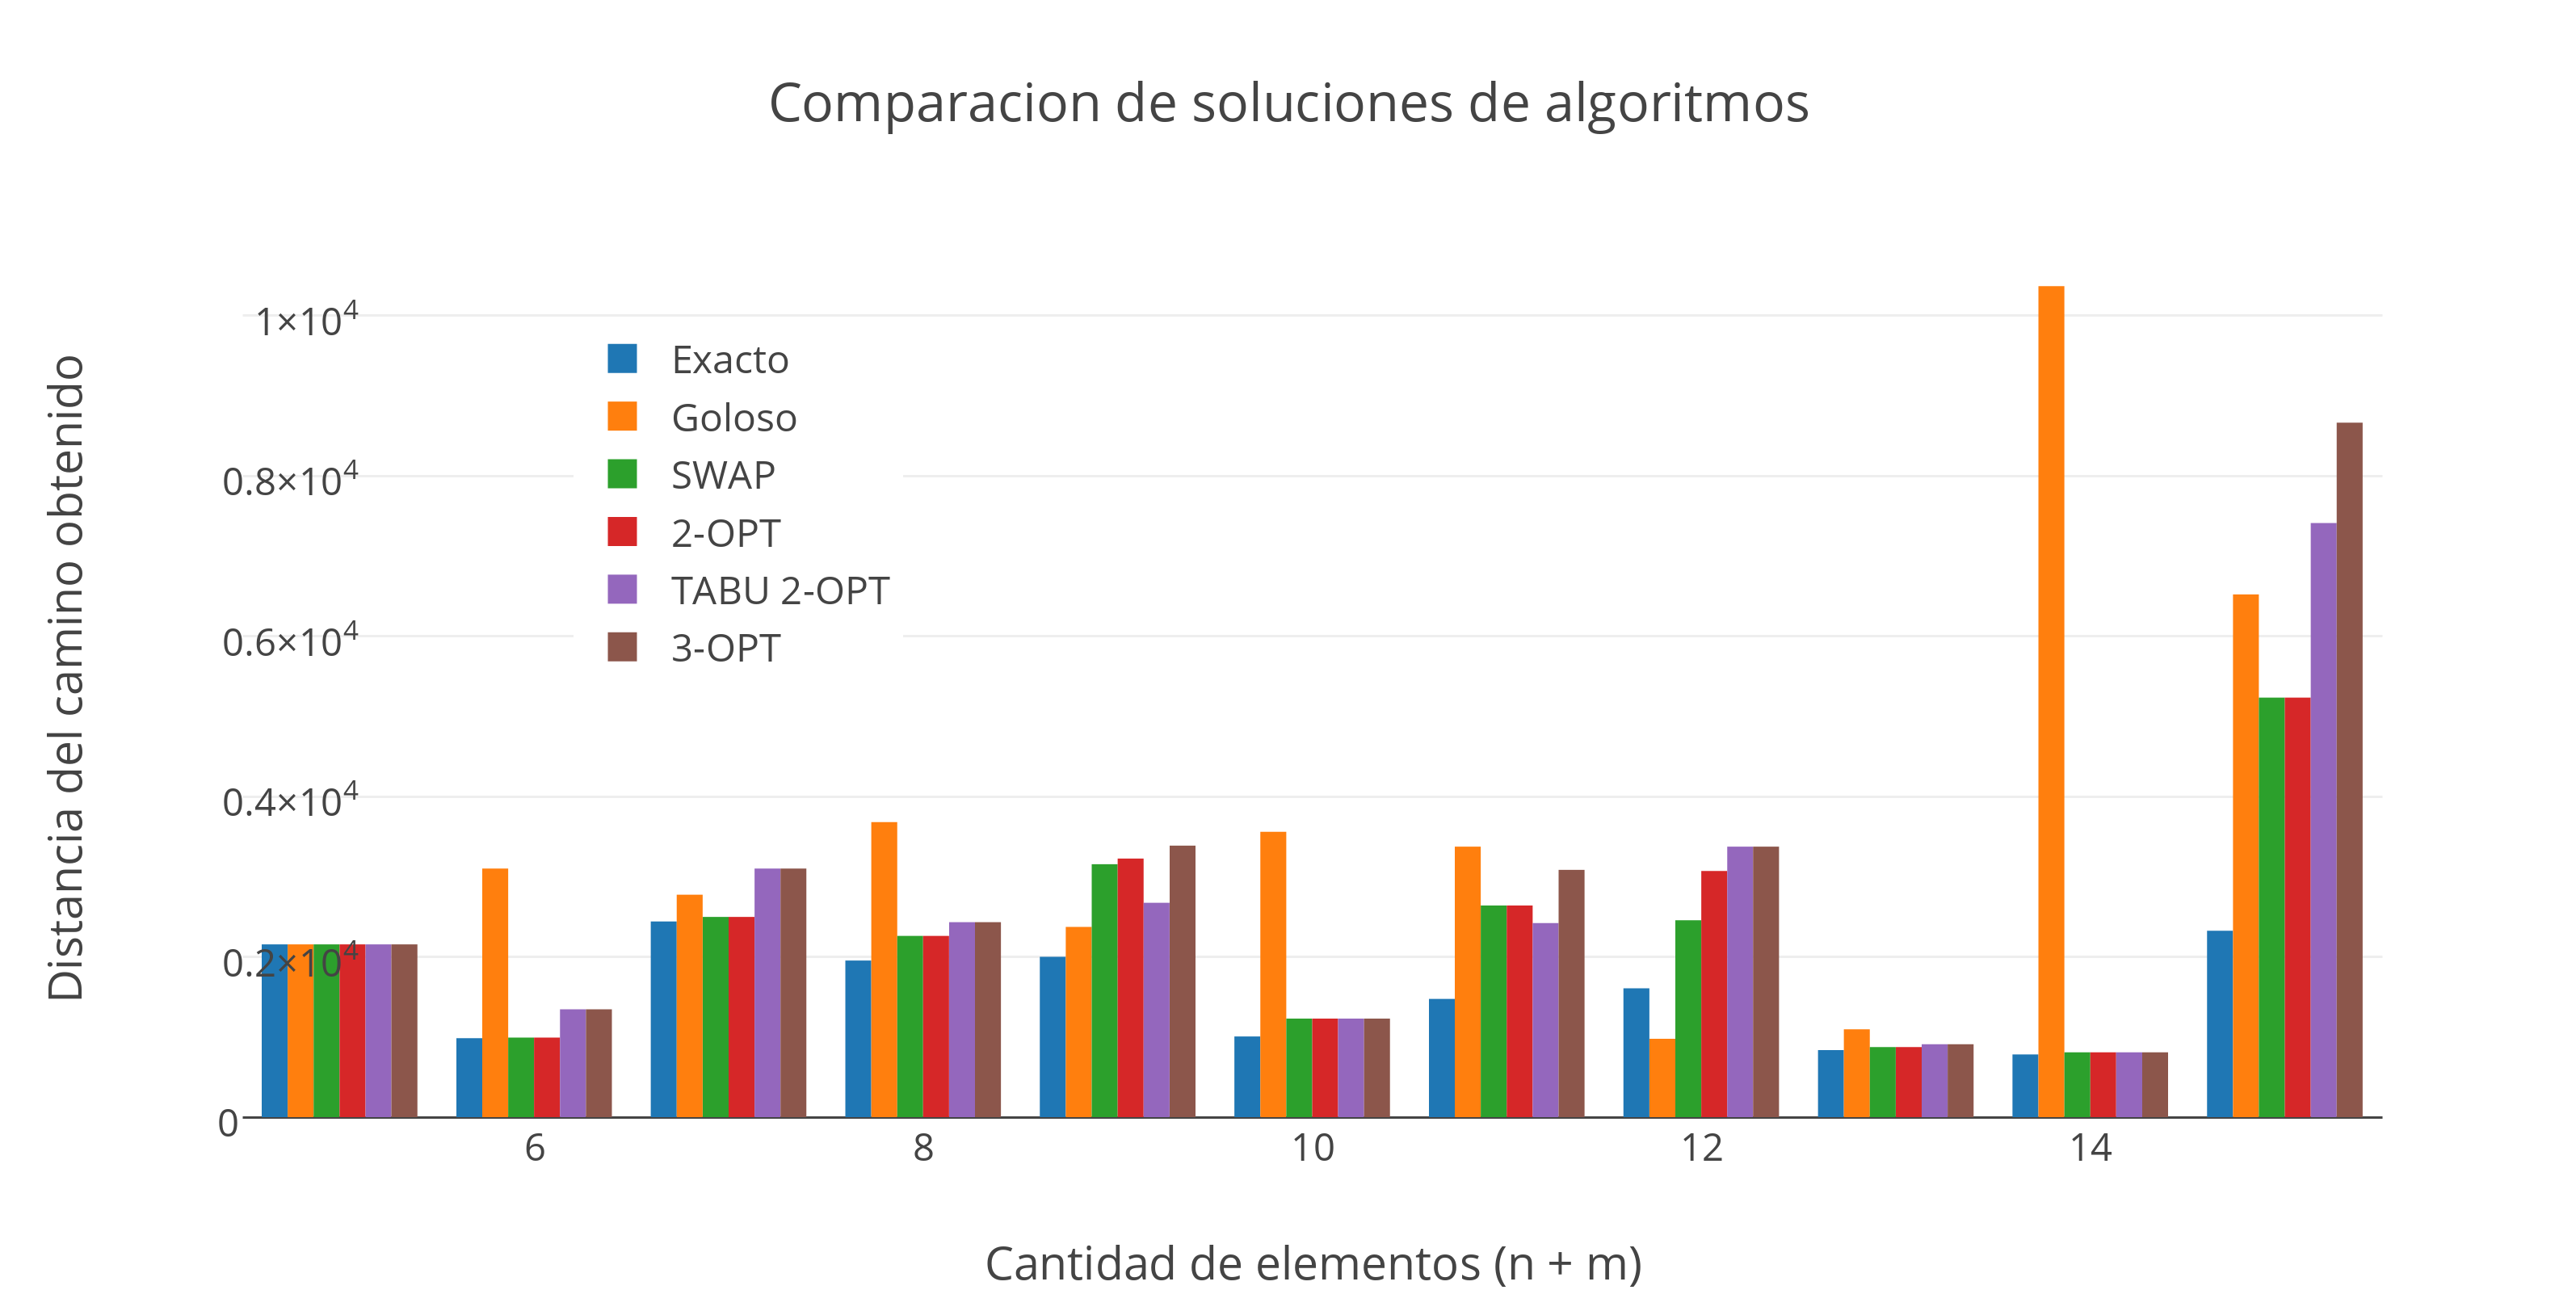
\includegraphics[scale=0.5]{./EJ5/comparativo2.png}\\
 {\textit{Gráfico \ 5.2 - Comparaci\'on de soluciones de todos los algoritmos}}
  \end{center}
  \vspace*{0.3cm}

\vspace*{0.3cm} \vspace*{0.3cm}
  \begin{center}
 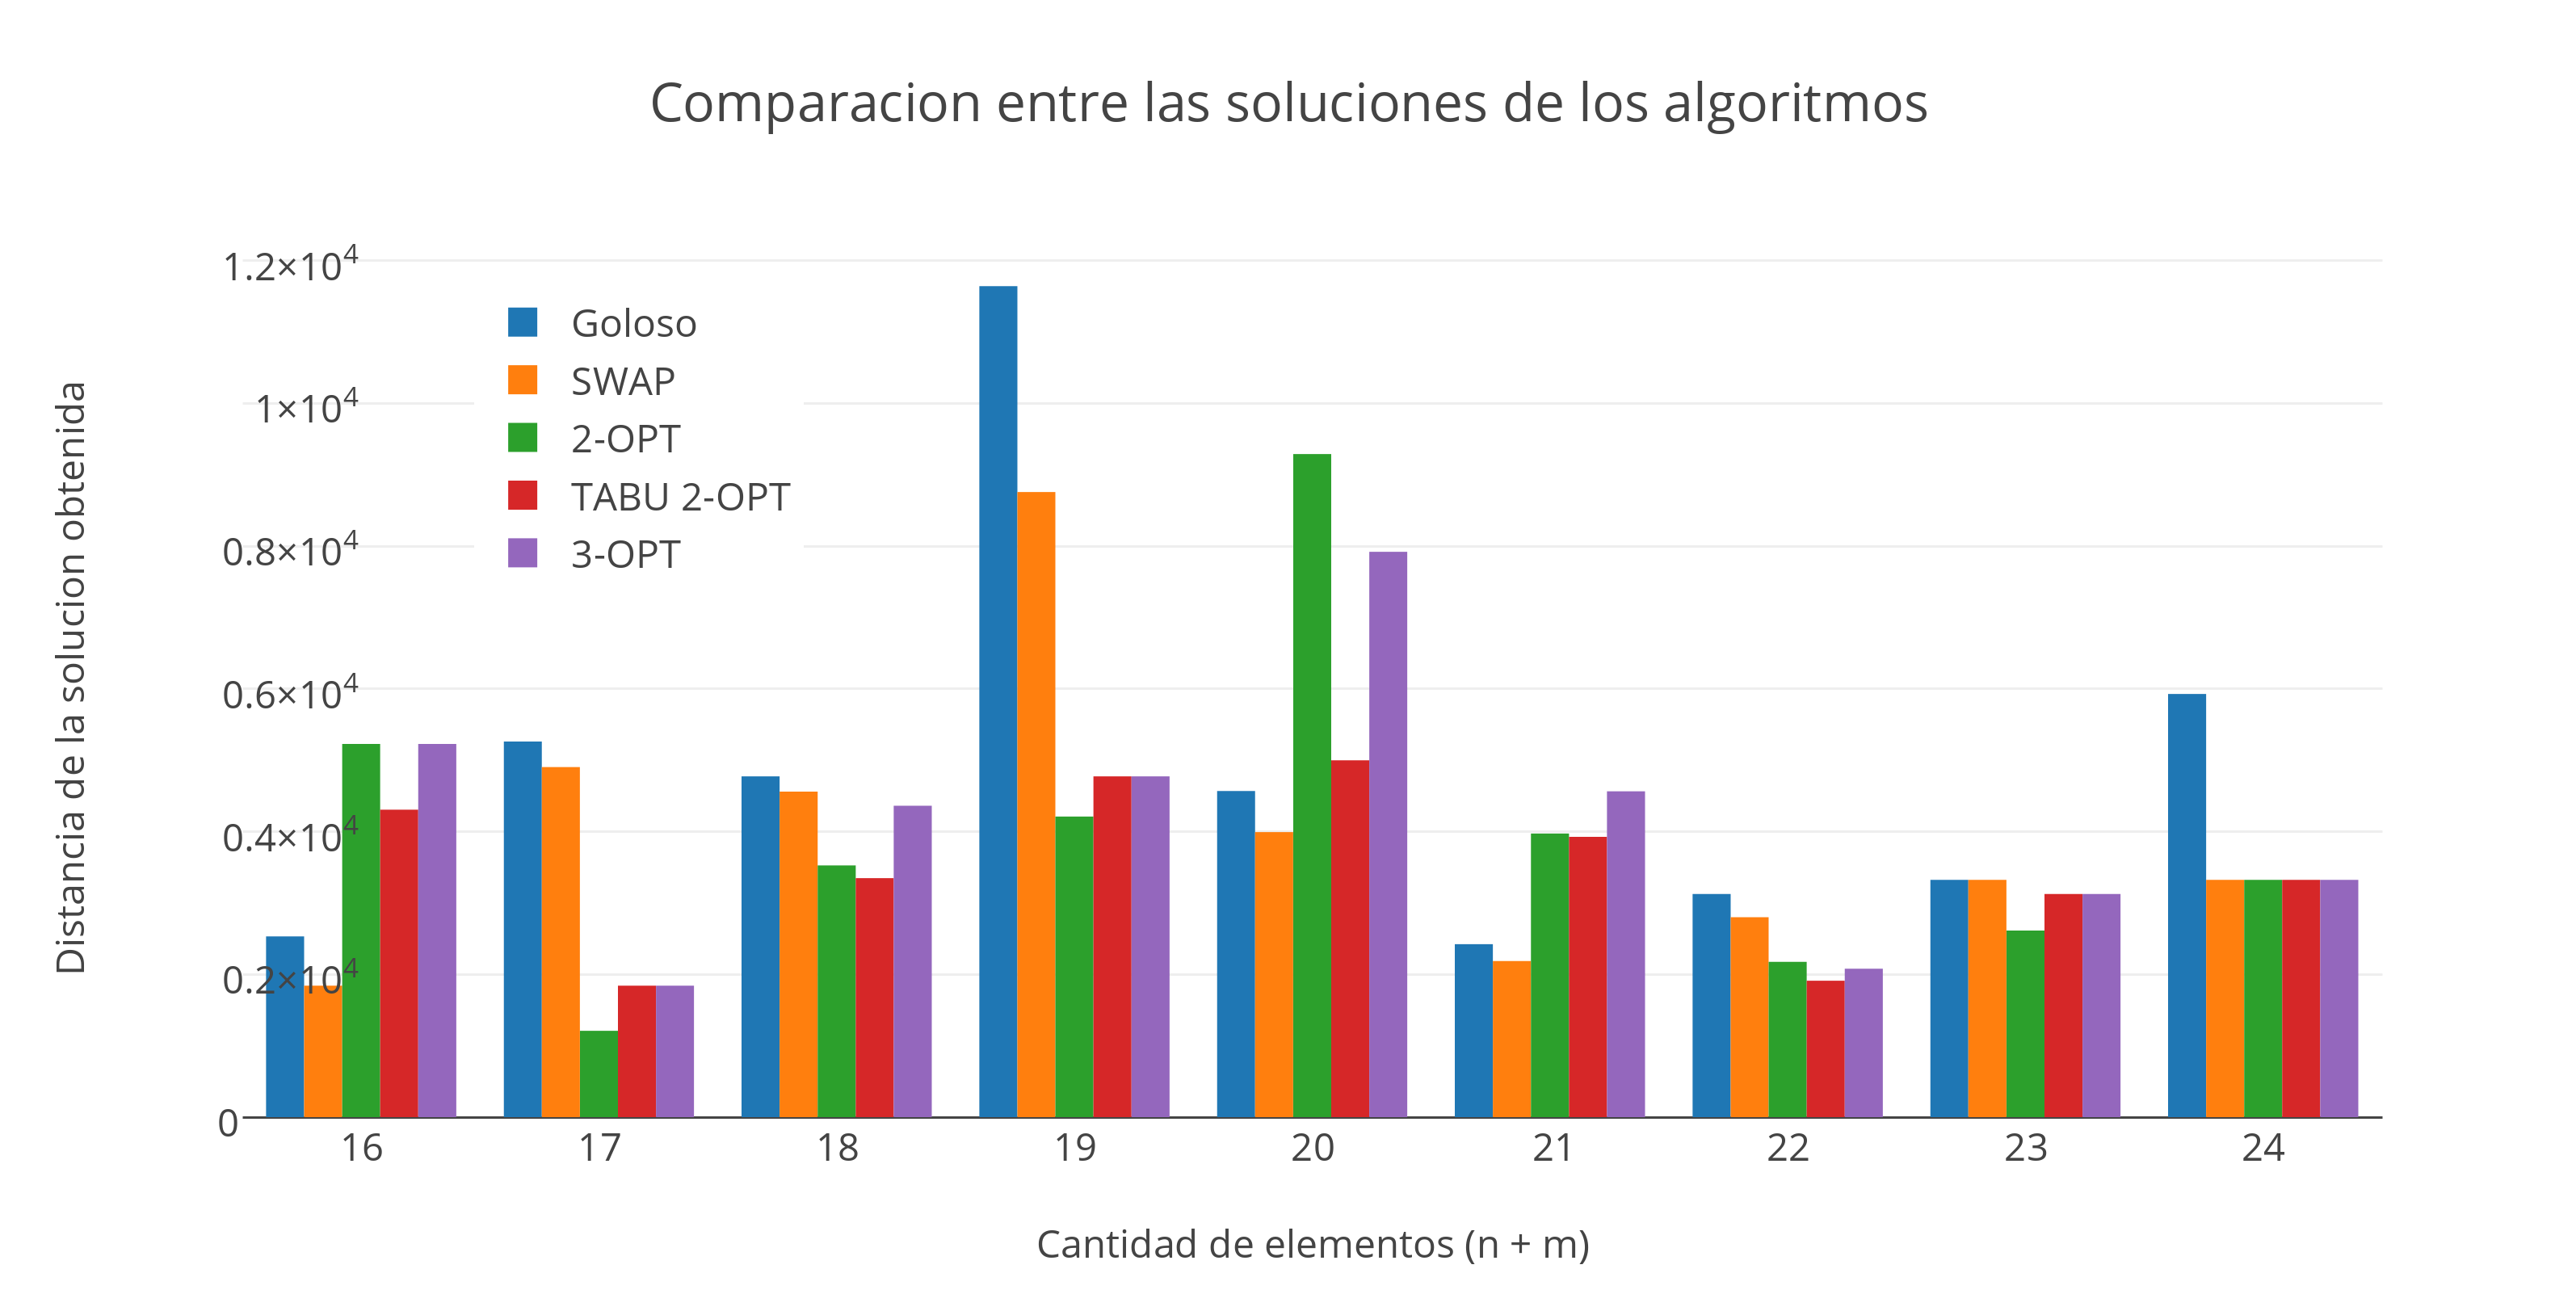
\includegraphics[scale=0.5]{./EJ5/comparativo1.png}\\
 {\textit{Gráfico \ 5.3 - Comparaci\'on de soluciones entre las heur\'isticas}}
  \end{center}
  \vspace*{0.3cm}


\subsubsection{Comparacion de calidad de solución}
INSERTAR GRAFICOS DE BOXPLOTS ENTRE LOS ERRORES DE CADA HEURISTICA:
	ERROR VS TAMAÑO DE ENTRADA POR CADA HEURISTICA (cada columna que forme un boxplot en el grafico comparativo)
	
	\vspace*{0.3cm} \vspace*{0.3cm}
  \begin{center}
 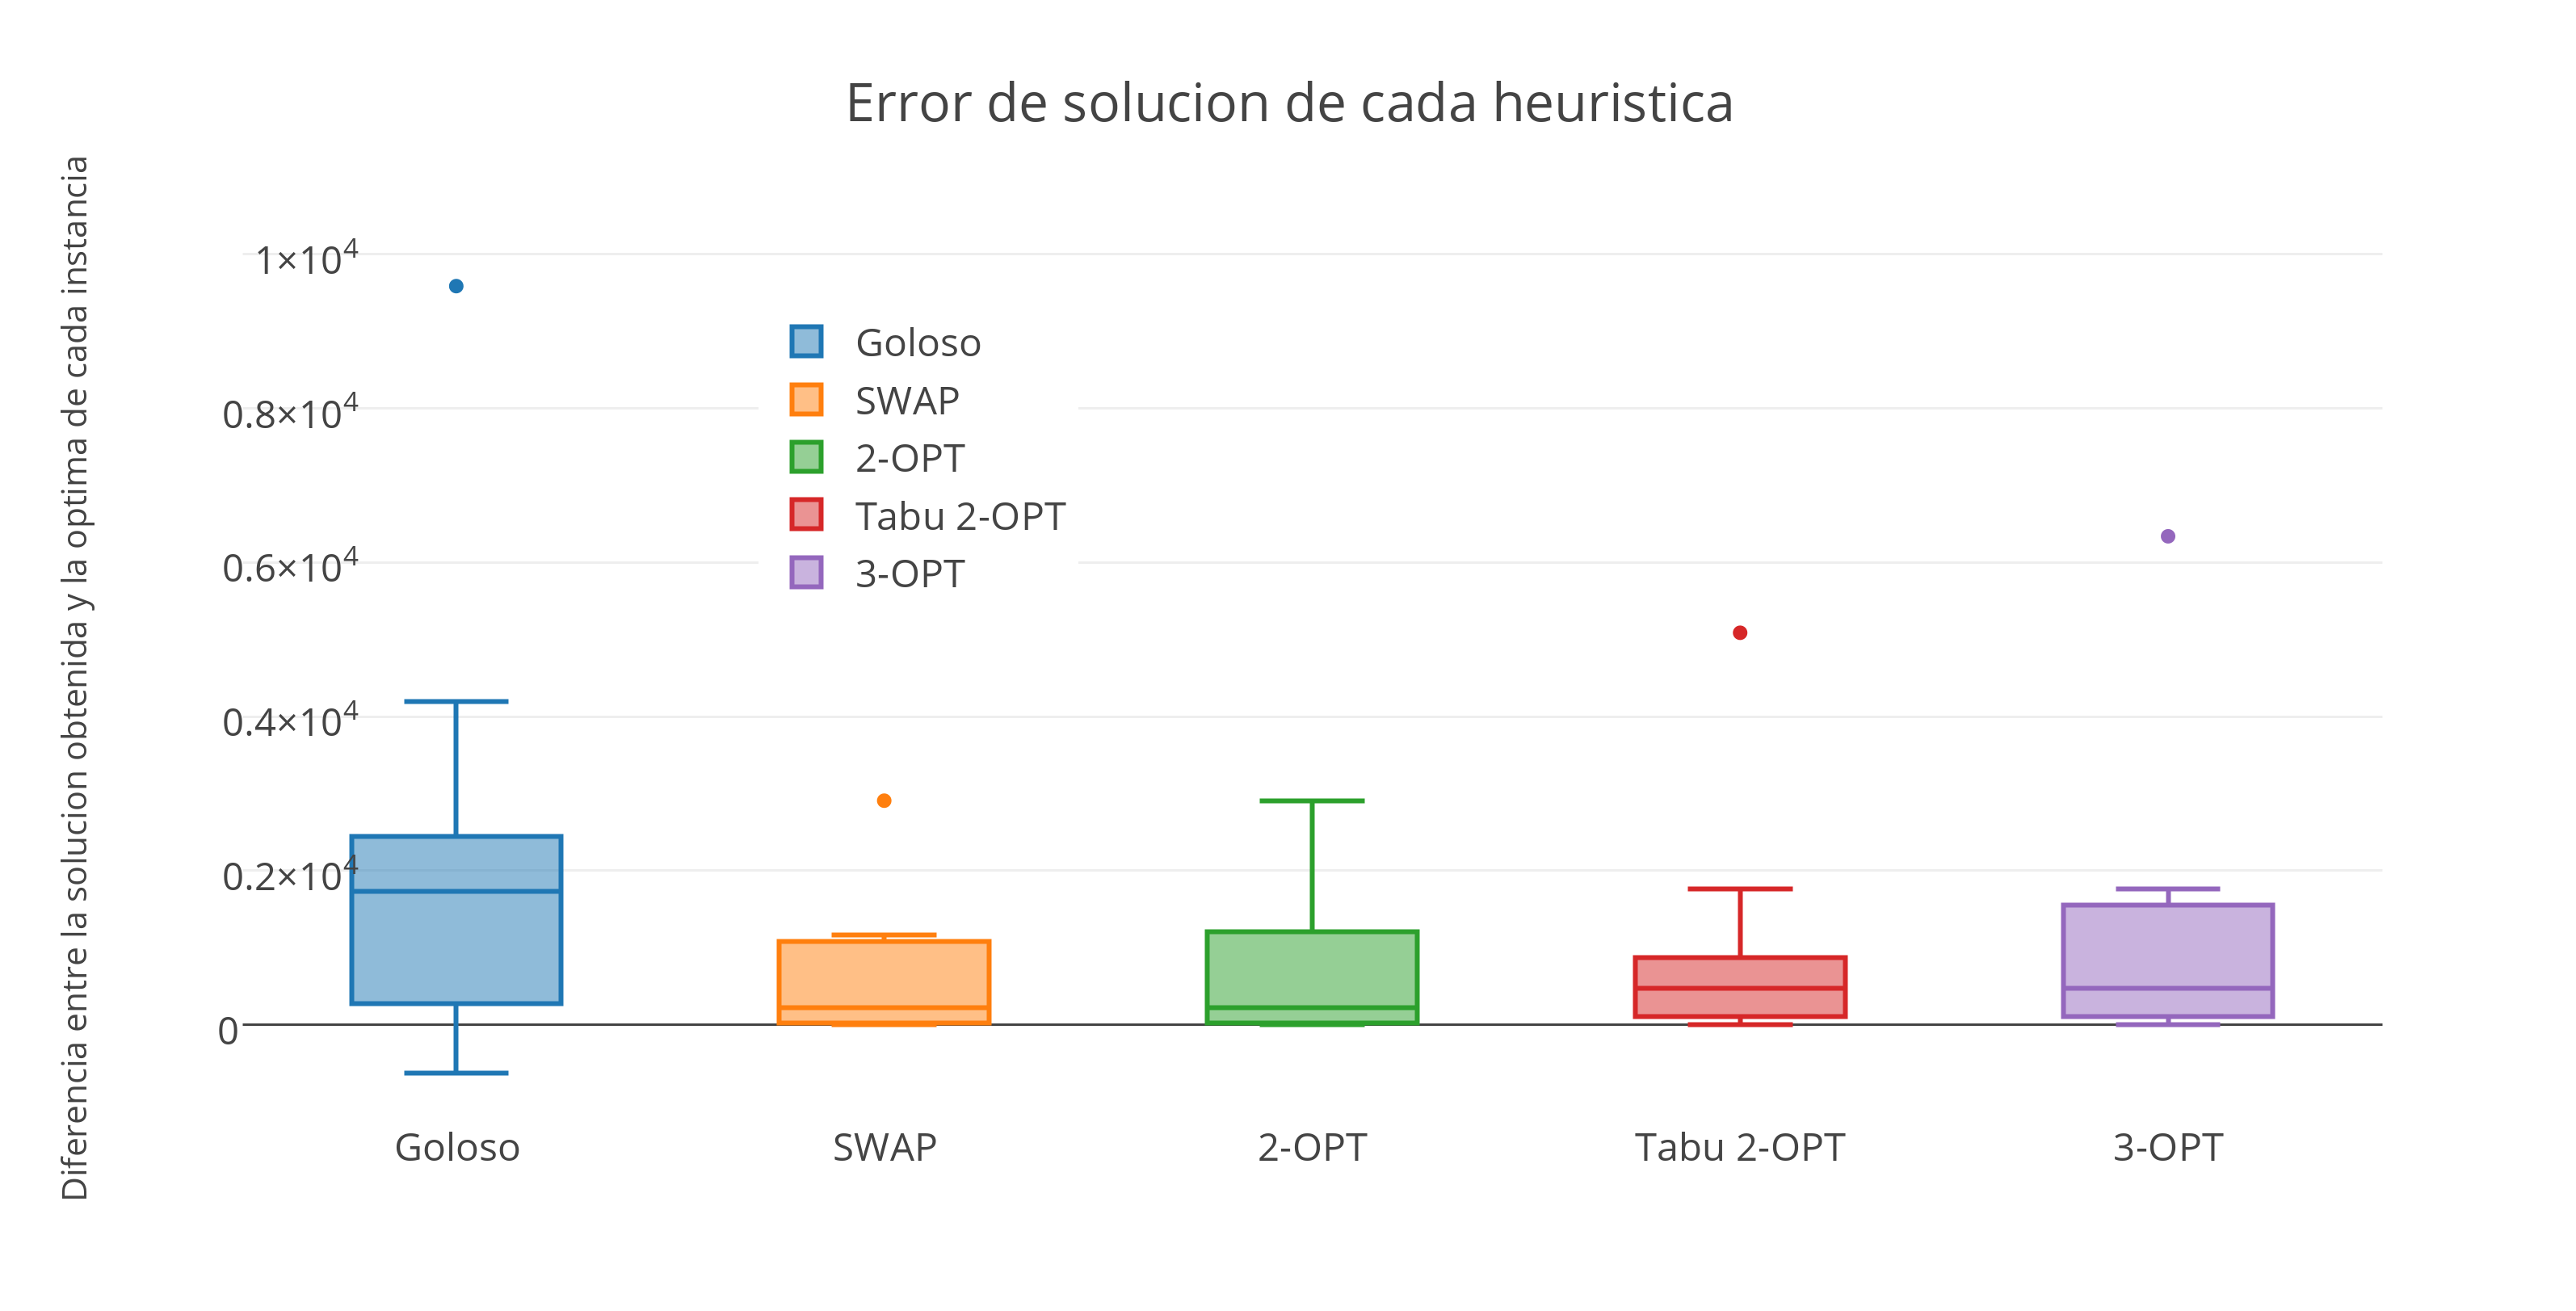
\includegraphics[scale=0.5]{./EJ5/errorporalgoritmo.png}\\
 {\textit{Gráfico \ 5.4 - Error en la soluciones de las heur\'isticas}}
  \end{center}
  \vspace*{0.3cm}
	
	-----> CHAMULLO ESTEBAN